% To remove when JSS.cls is fixed
% https://github.com/rstudio/rticles/issues/329
\RequirePackage[2020/02/02]{latexrelease}
\documentclass[
  shortnames]{jss}

\usepackage[utf8]{inputenc}

\providecommand{\tightlist}{%
  \setlength{\itemsep}{0pt}\setlength{\parskip}{0pt}}

\author{
Shannon K. Gallagher\\Biostatistics Research Branch\\
National Institute of Allergy\\
and Infectious Diseases \And Benjamin Leroy\\Dept. of Statistics\\
Carnegie Mellon University
}
\title{Time invariant analysis of epidemics with \pkg{EpiCompare}}

\Plainauthor{Shannon K. Gallagher, Benjamin Leroy}
\Plaintitle{A Capitalized Title: Something about a Package foo}
\Shorttitle{\pkg{foo}: A Capitalized Title}

\Abstract{
The abstract of the article.
}

\Keywords{keywords, not capitalized, \proglang{Java}}
\Plainkeywords{keywords, not capitalized, Java}

%% publication information
%% \Volume{50}
%% \Issue{9}
%% \Month{June}
%% \Year{2012}
%% \Submitdate{}
%% \Acceptdate{2012-06-04}

\Address{
    Shannon K. Gallagher\\
    Biostatistics Research Branch\\
National Institute of Allergy\\
and Infectious Diseases\\
    5603 Fishers Lane\\
Rockville, MD 20852\\
  E-mail: \email{shannon.gallagher@nih.gov}\\
  URL: \url{http://skgallagher.github.io}\\~\\
      Benjamin Leroy\\
    Dept. of Statistics\\
Carnegie Mellon University\\
    5000 Forbes Ave.\\
Pittsburgh, PA 15213\\
  E-mail: \email{bpleroy@andrew.cmu.edu}\\
  URL: \url{https://benjaminleroy.github.io/}\\~\\
  }

% Pandoc citation processing

% Pandoc header
\usepackage{booktabs}
\usepackage{longtable}
\usepackage{array}
\usepackage{multirow}
\usepackage{wrapfig}
\usepackage{float}

\usepackage{amsmath}

\begin{document}

\section{Introduction}\label{sec:intro}

This is the Section \ref{sec:intro}. This template demonstrates some of
the basic LaTeX that you need to know to create a JSS article.

\hypertarget{code-formatting}{%
\subsection{Code formatting}\label{code-formatting}}

In general, don't use Markdown, but use the more precise LaTeX commands
instead:

\begin{itemize}
\item
  \proglang{Java}
\item
  \pkg{plyr}
\end{itemize}

One exception is inline code, which can be written inside a pair of
backticks (i.e., using the Markdown syntax).

If you want to use LaTeX commands in headers, you need to provide a
\texttt{short-title} attribute. You can also provide a custom identifier
if necessary. See the header of Section \ref{r-code} for example.

\section[R code]{\proglang{R} code}\label{r-code}

Can be inserted in regular R markdown blocks.

hags hags hags \cite{Neal2004}

\begin{CodeChunk}
\begin{CodeInput}
R> x <- 1:10
R> x
\end{CodeInput}
\begin{CodeOutput}
 [1]  1  2  3  4  5  6  7  8  9 10
\end{CodeOutput}
\end{CodeChunk}

\section[Tour]{A tour of \pkg{EpiCompare}}\label{sec:tour}

In this section, we highlight a number of the functionalities available
in \proglang{EpiCompare}. These functionalities include data cleaning,
visualization, simulation, and comparison, in accordance with the data
analysis pipeline REF\ref{}. We show a full data analysis from beginning
to end that can be accomplished in a streamlined and standardized
manner.

\subsection{Data and exploratory analysis}

We analyze an outbreak of measles in the town of Hagelloch, Germany from
1861-1862, a data set organized by \cite{pfeilsticker1863}. The data was
later made visible by \cite{oesterle1992} and made available in an
\proglang{R} by \cite{surveillance2017}. The Hagelloch data includes a
rich set of features including household members, school level,
household locations, date of first symptoms (prodromes), date of measles
rash, and even the alleged infector. A subset of the data is shown in
Table \ref{tab:hags-people} Because of these rich features, this data
set has been an ideal testing ground methodology in infectious disease
epidemiology and is used in work by
\cite{Neal2004,britton2011,groendyke2012,becker2016}.

After loading in the libraries for this analysis, we examine . Within
it, we

\begin{CodeChunk}
\begin{table}[!h]

\caption{\label{tab:hags-people}Subset of Hagelloch infection data.  Features include the person ID, household ID (HH ID), age, sex, class level (Pre-K/1st/2nd), date of first symptoms, date of the appearance of the measles rash, and the alleged infector ID of the individual.}
\centering
\begin{tabular}[t]{rrlrllllr}
\toprule
ID & HH ID & Name & Age & Sex & Class & Symp. Start & Rash Date & Infector ID\\
\midrule
1 & 61 & Mueller & 7 & female & 1st class & 1861-11-21 & 1861-11-25 & 45\\
2 & 61 & Mueller & 6 & female & 1st class & 1861-11-23 & 1861-11-27 & 45\\
3 & 61 & Mueller & 4 & female & preschool & 1861-11-28 & 1861-12-02 & 172\\
4 & 62 & Seibold & 13 & male & 2nd class & 1861-11-27 & 1861-11-28 & 180\\
5 & 63 & Motzer & 8 & female & 1st class & 1861-11-22 & 1861-11-27 & 45\\
45 & 51 & Goehring & 7 & male & 1st class & 1861-11-11 & 1861-11-13 & 184\\
\bottomrule
\end{tabular}
\end{table}

\end{CodeChunk}

With \pkg{EpiCompare}, we can easily obtain the empirical cumulative
incidence function with respect to the measles rash appearance (variable
\code{ERU}) with the following tidy-style function,
\code{agents_to_aggregate}. The function \code{agents_to_aggregate} is a
key component of \pkg{EpiCompare}, allowing the user to easily switch
from an individual-level (i.e.~an agent) view of a disease to an
aggregate level. For example, the below code shows how we can convert
the agent data to a cumulative incidence of the measles rash, in order
to see how the disease spread through the population over time. We can
then compare the cumulative incidence of the rash to the cumulative
incidence of the prodromes, i.e.~the initial symptoms. We do this with
the below code, and a part of the cumulative incidence data output are
shown in Table \ref{tab:cif-rash}. The argument
\code{integer_time_expansion} indicates whether we should include all
time points in the recorded range of the data or only when there is a
change in the incidence.

\begin{CodeChunk}
\begin{CodeInput}
R> cif_rash  <- hagelloch_raw %>%
+   mutate(time_of_rash = as.numeric(ERU - min(PRO, na.rm = TRUE))) %>%
+   agents_to_aggregate(states = time_of_rash,
+                       integer_time_expansion = FALSE) %>%
+   mutate(type = "Rash")
\end{CodeInput}
\end{CodeChunk}

\begin{CodeChunk}
\begin{table}[!h]

\caption{\label{tab:cif-rash}Turning the individual-level information from the Hagelloch data to an aggregate view of the cumulative incidence of the measles rash in the population over time.}
\centering
\begin{tabular}[t]{rrr}
\toprule
Time & \# Susceptible & \# Total rash appearances\\
\midrule
0 & 188 & 0\\
4 & 187 & 1\\
7 & 186 & 2\\
9 & 185 & 3\\
12 & 183 & 5\\
\bottomrule
\end{tabular}
\end{table}

\end{CodeChunk}

One question of interest is the duration between initial onset of
prodromes or symptoms and the appearance of the measles rash. Since
\code{agent_to_aggregate} outputs a tidy-style data frame, it is a
simple task to plot the two sets of incidence curves on the same graph
(Fig. \ref{fig:cifs}).

\begin{CodeChunk}
\begin{CodeInput}
R> cif_prodromes <- hagelloch_raw %>%
+   mutate(time_of_PRO = as.numeric(PRO - min(PRO, na.rm = TRUE))) %>%
+   agents_to_aggregate(states = time_of_PRO,
+                       integer_time_expansion = FALSE) %>%
+   mutate(type = "Pro")
\end{CodeInput}
\end{CodeChunk}

\begin{CodeChunk}
\begin{CodeInput}
R> plot_df <- bind_rows(cif_rash, cif_prodromes)
R> 
R> ggplot(data = plot_df,
+        aes(x = t, y = X1, col = type)) + 
+   geom_step() + 
+   labs(title = "Cumulative incidence of measles appearance",
+        x = "Time (days relative to first prodrome appearance)",
+        y = "Cumulative incidence of event") + 
+   coord_cartesian(xlim = c(0, 55)) +
+   scale_color_manual(values = c("blue", "red"))
\end{CodeInput}
\begin{figure}[H]

{\centering 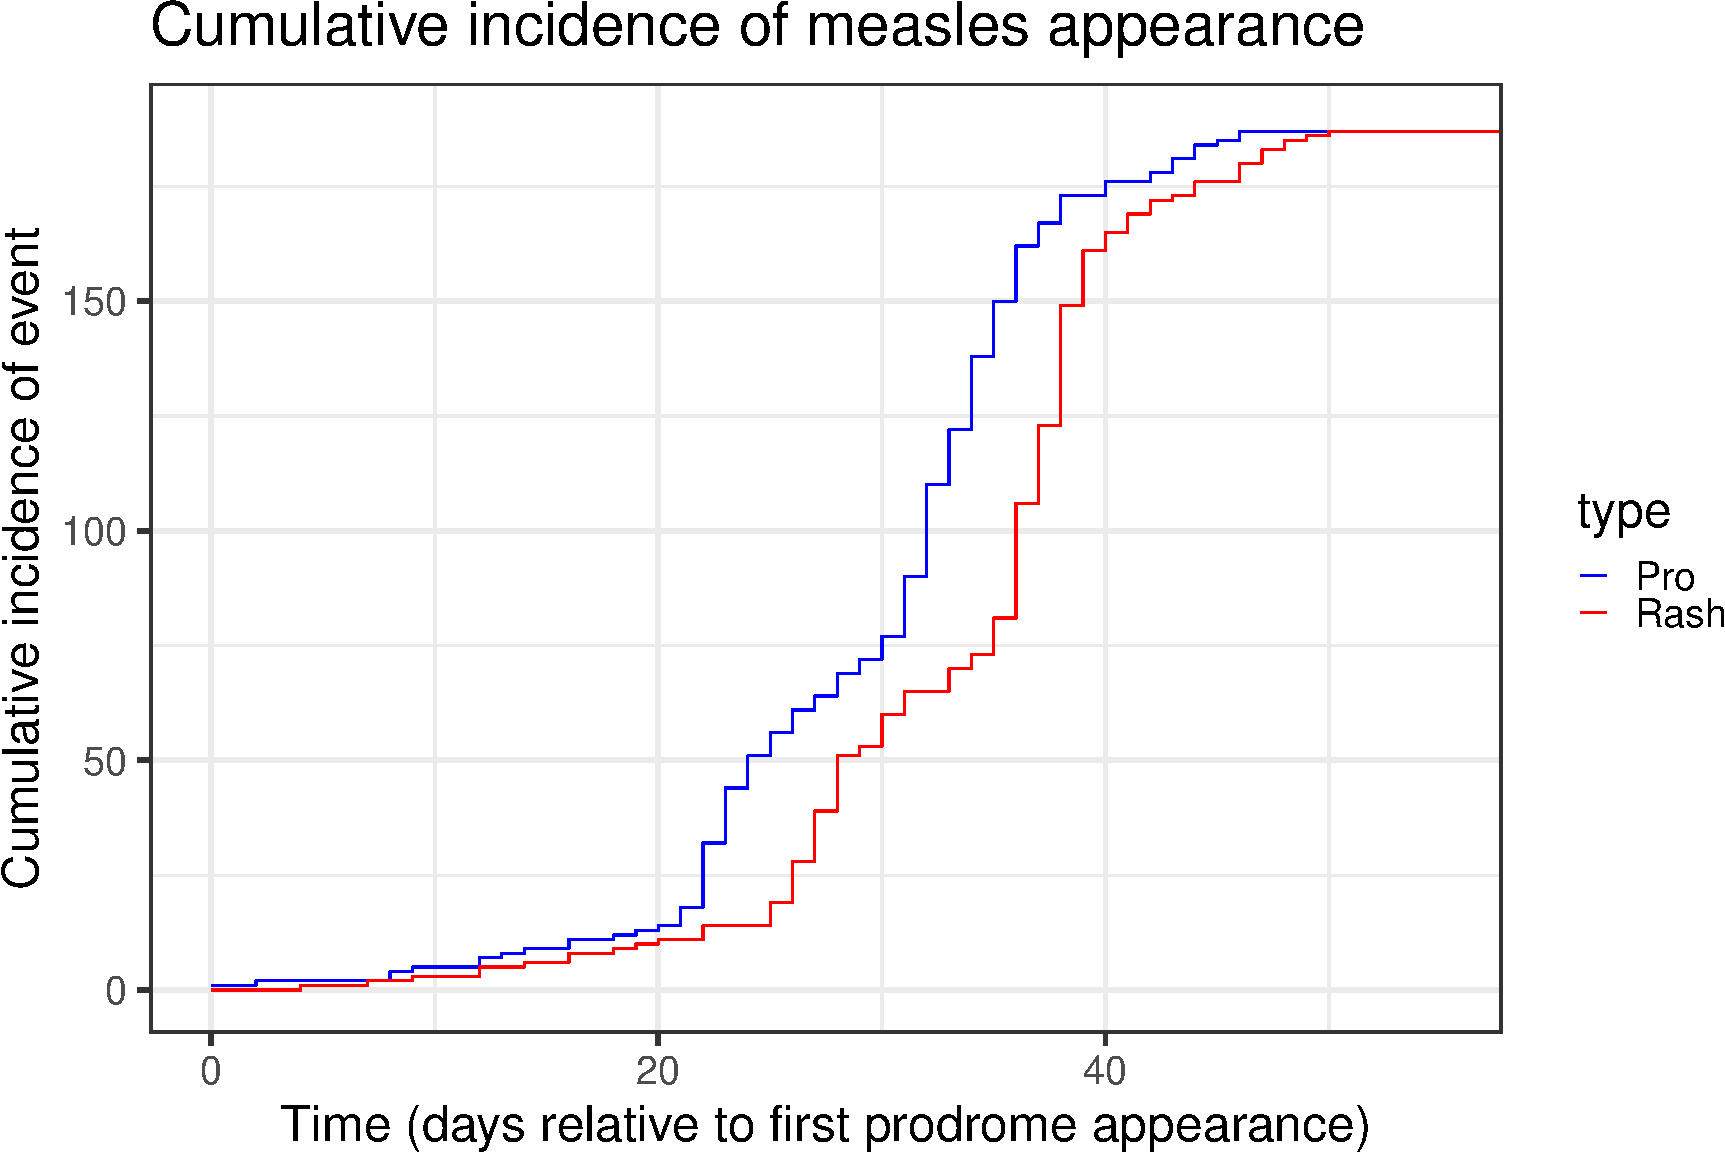
\includegraphics{Figs/unnamed-chunk-6-1} 

}

\caption{\label{fig:cifs}Empirical cumulative incidence functions of prodrome (symptom) onset and measles rash appearance.  We see that there is approximately a a constant lag between the two curves.}\label{fig:unnamed-chunk-6}
\end{figure}
\end{CodeChunk}

\begin{CodeChunk}
\begin{CodeInput}
R> with(hagelloch_raw, sum(PRO > ERU, na.rm = TRUE))
\end{CodeInput}
\begin{CodeOutput}
[1] 0
\end{CodeOutput}
\end{CodeChunk}

The real power of \code{agents_to_aggregate()} lies in its ability to
aggregate over any number of pre-specified states. For example, the
Hagelloch data sets contains two columns, \code{tI} and \code{tR}, the
time of infection and recovery, respectively of each individual. We can
then plot the SIR values through a time-invariant lens via a ternary
plot using regular \pkg{ggplot2} functions or with our custom
\code{geom}, \code{geom_aggregate}, which takes the original agent data
as input (\ref{fig:hag-tern-raw}.

\begin{CodeChunk}
\begin{CodeInput}
R> sir <- hagelloch_raw %>%
+   agents_to_aggregate(states = c(tI, tR),
+                       min_max_time = c(0, 55)) %>%
+   rename(time = t, S = X0, I = X1, R = X2)
R> 
R> 
R> ggplot(sir, aes(x = S, y = I, z = R))+
+   coord_tern() +
+   geom_path() +
+   labs(x = "S", y = "I", z = "R",
+        title = "Time invariant view of Hagelloch measles outbreak") + 
+   theme_sir()
\end{CodeInput}
\begin{figure}[H]

{\centering 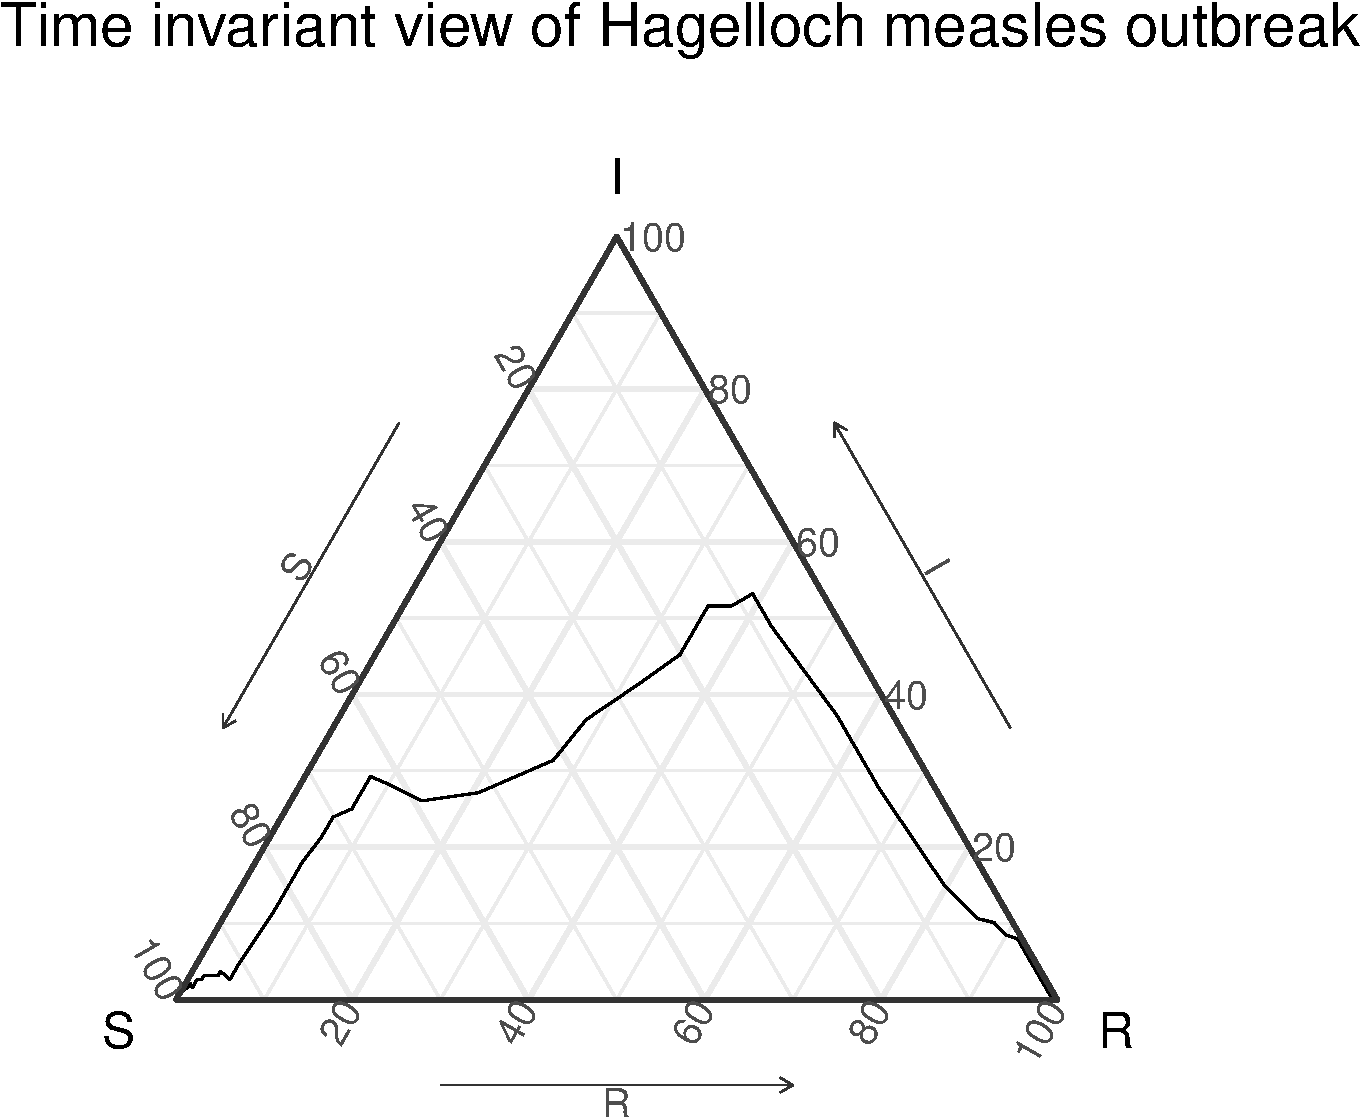
\includegraphics{Figs/unnamed-chunk-8-1} 

}

\caption{\label{fig:hag-tern-raw}Time invariant view of the Hagelloch epidemic where we view the individuals in Susceptible, Infectious, or Recovered states.  We see there are two peaks of infection (the vertical axis).}\label{fig:unnamed-chunk-8}
\end{figure}
\end{CodeChunk}

Moreover, we can look at the outbreaks of the disease by group within
\code{agent_to_aggregate()} or \code{geom_aggregate()}, which allows us
to examine differences among the groups of individuals. For example, we
show the time invariant outbreak by class level in Figure
\ref{fig:tern-class-data}. Immediately, we see that time invariant
infection curve is very different for the pre-school group compared to
the 1st class. In the 1st class, we see about 95\% of the class become
infected before anyone recovers, which is indicative of a
super-spreading event. This suspicion is further confirmed in that 26 of
the 30 have been reportedly infected by the same individual.

\begin{CodeChunk}
\begin{CodeInput}
R> hagelloch_raw %>%
+   ggplot(aes(y = tI, z = tR, color = CL)) +
+   geom_aggregate(size = 2) + coord_tern() +
+   labs(x = "S", y = "I", z = "R",
+        color = "Class") +
+   scale_color_brewer(palette = "Dark2") +
+   facet_wrap(~CL)
\end{CodeInput}
\begin{figure}[H]

{\centering 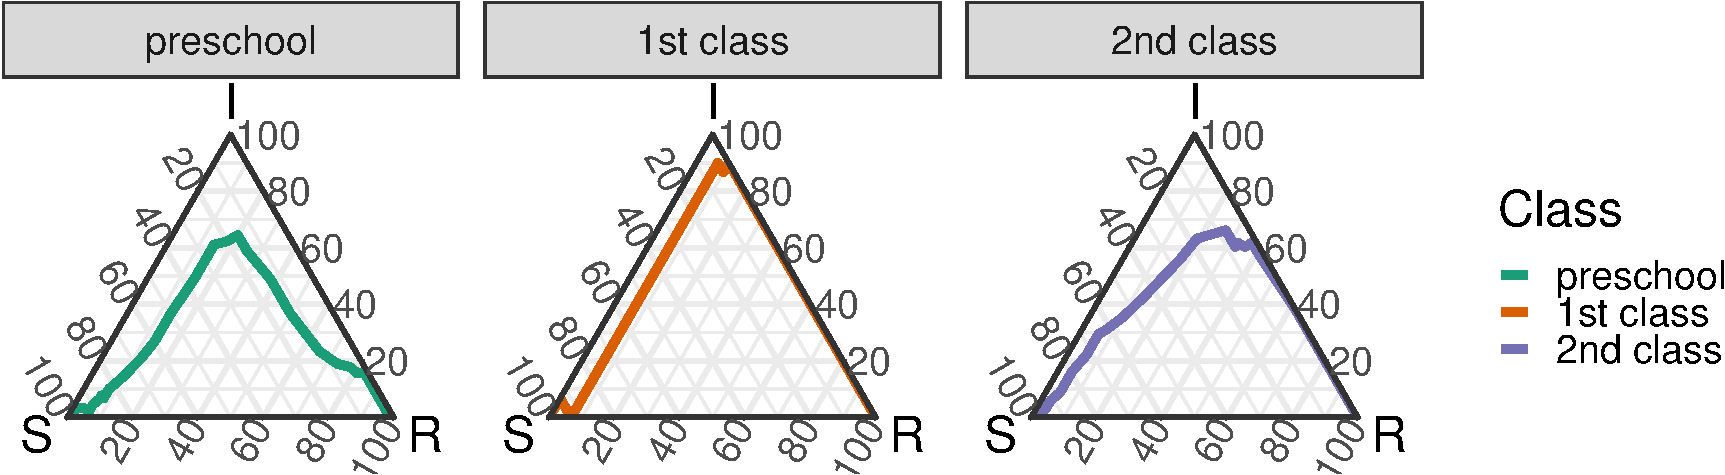
\includegraphics{Figs/unnamed-chunk-9-1} 

}

\caption{\label{fig:tern-class-data}Time invariant outbreak curves for the three class groups.  The pre-school class has a distinct peak of infection whereas the peak infection point for the other two classes are less well defined.}\label{fig:unnamed-chunk-9}
\end{figure}
\end{CodeChunk}

\begin{itemize}
\item thing
\end{itemize}

\bibliography{EpiCompare.bib}


\end{document}
